\documentclass[11pt]{article}

\usepackage{graphicx}
\usepackage{courier}
\usepackage{underscore}

\title{Turing Machine Documentation}
\author{Adam Yedidia}

\begin{document}
    
\maketitle

This document explains the structure of the Turing machines used in this project. It is intended for users who are curious about the algorithm. Note that this document also appears nearly verbatim in Section 8 (Compilation and Processing) at:  \\ \\
\texttt{parsimony/tex/busybeaver/busybeaver.pdf} \\

There are two ways to think about the layout of the tape symbols: with a $4$-symbol alphabet ($\{\texttt{\_}, \texttt{1}, \texttt{H}, \texttt{E}\}$, blank symbol \texttt{\_}), and with a $2$-symbol alphabet ($\{\texttt{a}, \texttt{b}\}$, blank symbol \texttt{a}). \ The $2$-symbol alphabet version is the one that's ultimately used for the results in this paper, since we advertised a Turing machine that used only two symbols. \ However, in nearly all parts of the Turing machine, the $2$-symbol version of the machine is a direct translation of the $4$-symbol version, according to the following mapping:

\begin{itemize}
\item $\texttt{\_} \leftrightarrow \texttt{aa}$
\item $\texttt{1} \leftrightarrow \texttt{ab}$
\item $\texttt{H} \leftrightarrow \texttt{ba}$
\item $\texttt{E} \leftrightarrow \texttt{bb}$
\end{itemize}

The sections that follow sometimes refer to the \texttt{ERROR} state. \ Transitions to the \texttt{ERROR} state should never be taken under any circumstances, and are useful for debugging purposes.

\section{Concept} \label{sec:ontape}

A directory of TMD functions is converted at compilation time to a string of bits to be written onto the tape, along with other states designed to interpret these bits. \ The resulting Turing machine has three main components, or \emph{submachines}:

\begin{enumerate}
\item The \emph{initializer} sets up the basic structure of the variable registers and the function stack.
\item The \emph{printer} writes down the binary string that corresponds to the compiled TMD code.
\item The \emph{processor} interprets the compiled binary, modifying the variable registers and the function stack as necessary.
\end{enumerate}

The Turing machine's control flow proceeds from the initializer to the the printer to the interpreter. \ In other words, initializer states point only to initializer states or to printer states, printer states point only to printer states or to interpreter states, and interpreter states point only to interpreter states or the \texttt{HALT} state.

This division of labor, while seemingly straightforward, actually constitutes an important idea. \ The problem of the compiler is to convert a higher-level representation---a machine with many tapes, a larger alphabet, and a function stack---to the lower-level representation of a machine with a single tape, a $2$-symbol alphabet and no function stack. \ The immediately obvious solution, and the one taught in every computability theory class as a proof of the equivalence of different kinds of Turing machines, is to have every ``state'' in the higher-level machine compile down to many states in the lower-level machine. %See Figure~\ref{fig:mttost} for a visual representation of what such a conversion might look like.

While simple, this approach is suboptimal in terms of the number of states. \ As is nearly always true when designing systems to be parsimonious, the clue that improvement is possible lies in the presence of repetition. \ Each state transition in the higher-level machine is converted to a group of lower-level states with the same basic structure. \ Why not instead explain how to perform this conversion exactly once, and then apply the conversion many times?

This idea is at the core of the division of labor described previously. We begin by writing a description of the higher-level machine onto the tape, and then ``run'' the higher-level machine by reading what is on the tape with a set of states that understands how to interpret the encoded higher-level machine. We refer to this idea as \emph{on-tape processing}. The printer writes the TMD program onto the tape, and the processor executes it. As a result of using this scheme, we incur a constant \emph{additive} overhead---we have to include the processor in our final Turing machine---but we avoid the constant \emph{multiplicative} overhead required for the na\"ive scheme.

The subsections that follow describe each of the three submachines---the initializer, the printer, and the processor---in greater detail.

\section{The Initializer}

The initializer starts by writing a counter onto the tape which encodes how many registers there will be in the program. \ Using the value in that counter, it creates each register, with demarcation patterns between registers, and unique identifiers for each register. \ Each register's value begins with the pattern of non-blank symbols laid out in the \texttt{initvar} file. \ The initializer also creates the program counter, which starts at 0, and the function stack, which starts out with only a single function call to the top function in the \texttt{functions} file.

Figure~\ref{fig:postinit} is a detailed diagram describing the tape's state when the initializer passes control to the printer.

\begin{figure}
\begin{center}
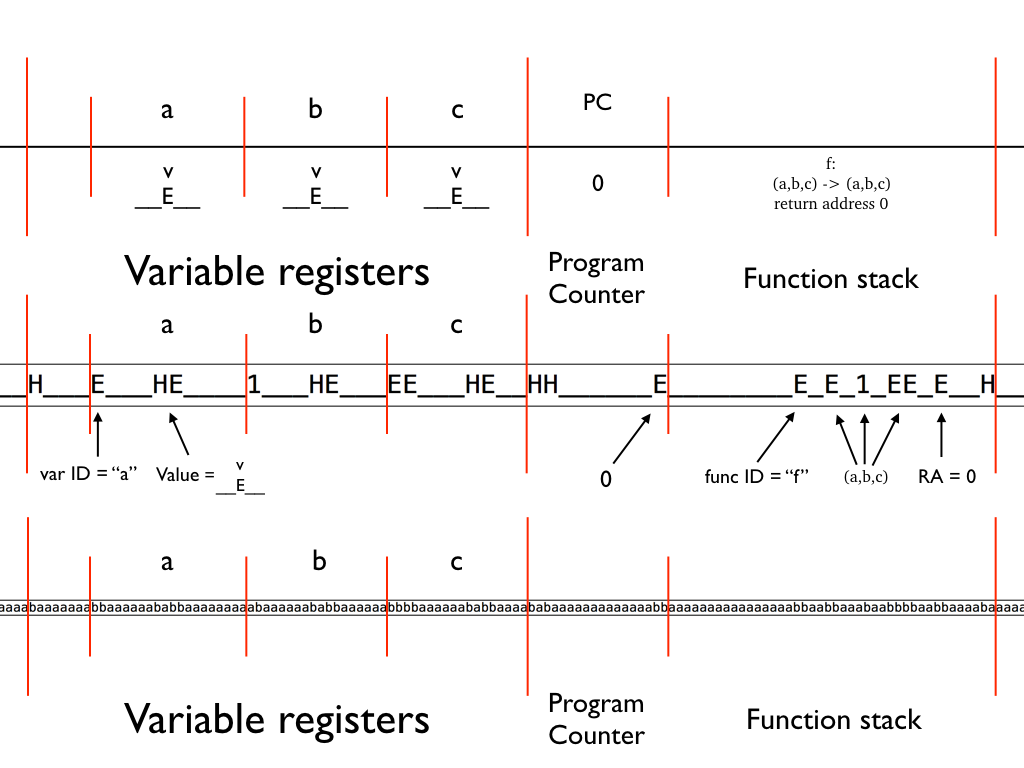
\includegraphics[scale=0.36]{figs/postinit.png}
\caption{The state of the Turing machine tape after the initializer completes. \ The top bar is a high-level description of what each part of the Turing machine tape represents. \ The middle bar is an encoding of the tape in the standard $4$-symbol alphabet; the bottom bar is simply the translation of that tape into the $2$-symbol alphabet. \label{fig:postinit}}
\end{center}
\end{figure}

\section{The Printer} \label{sec:introspect}

\subsection{Specification}

The printer writes down a long binary string which encodes the entirety of the TMD program onto the tape.

Figure~\ref{fig:postprog} shows the tape's state when the printer passes control to the processor.

\begin{figure}
\begin{center}
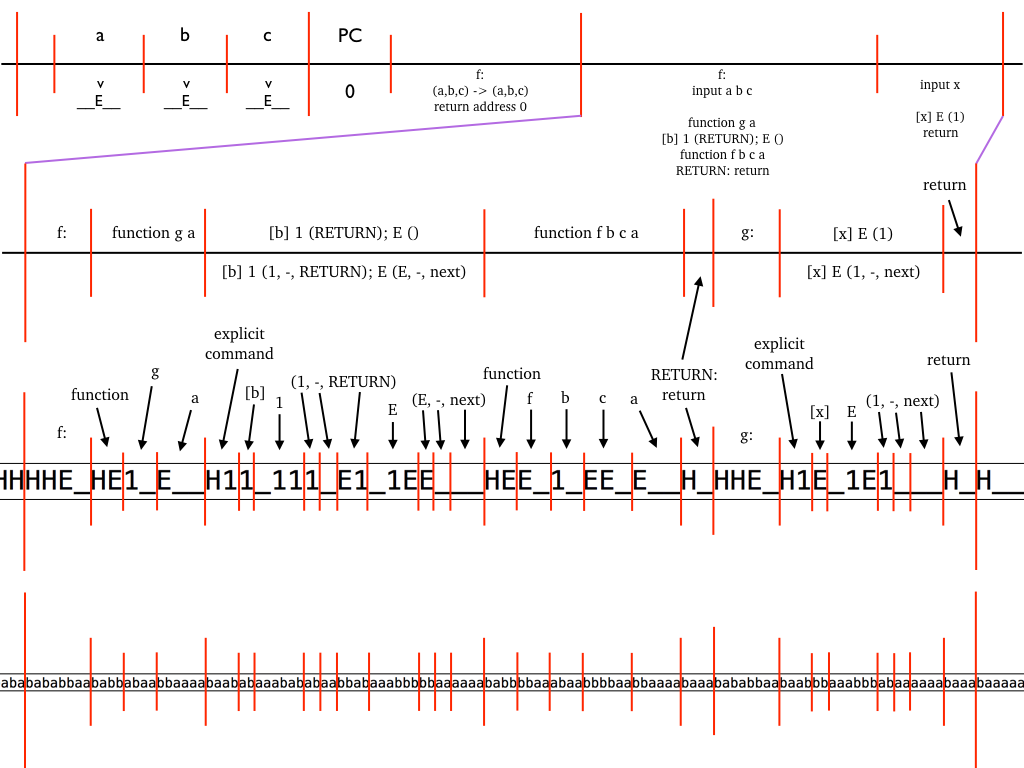
\includegraphics[scale=0.36]{figs/postprog.png}
\caption{The state of the Turing machine tape after the printer completes. \ The top bar is a high-level description of the entire tape; unfortunately, at this point there are so many symbols on the tape that it is impossible to see everything at once. \ For a detailed view of the first two-thirds of the tape (registers, program counter, and stack), see Figure~\ref{fig:postinit}. \ The bottom three bars show a zoomed-in view of the program binary. \ From the top, the second bar gives a high-level description of what each part of the program binary means; the third bar gives the direct correspondence between $4$-symbol alphabet symbols on the tape and their meaning in TMD; the fourth and final bar gives the translation of the third bar into the $2$-symbol alphabet. \label{fig:postprog}}
\end{center}
\end{figure}

\subsection{Introspection}

Writing down a long binary string onto a Turing machine tape in a parsimonious fashion is not as straightforward as it might initially appear. \ The first idea that comes to mind is simply to use one state per symbol, with each state pointing to the next, as shown in Figure~\ref{fig:naiveprog}.

\begin{figure}
\begin{center}
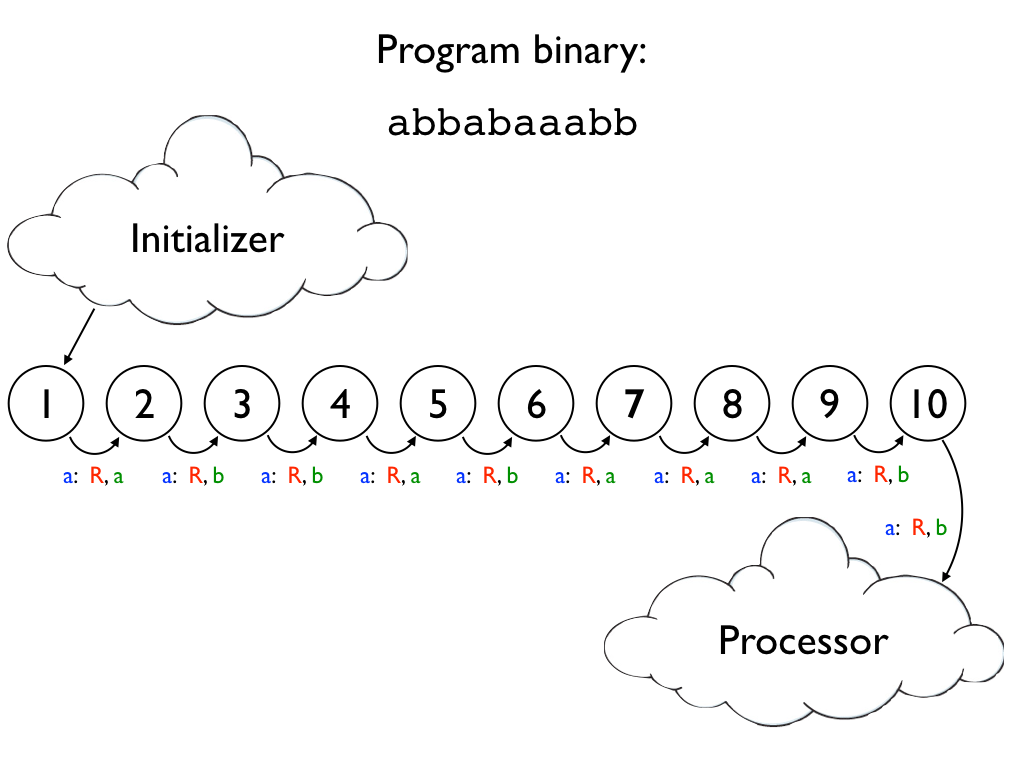
\includegraphics[scale=0.25]{figs/naiveprog.png}
\caption{A na\"ive implementation of the printer. \ In this example, the hypothetical program is ten bits long, and the printer uses ten states, one for each bit. \ In the diagram, the blue symbol is the symbol that is read on a transition, the red letter indicates the direction the head moves, and the green symbol indicates the symbol that it written. \ Note the lack of transitions on reading a \texttt{b}; this is because in this implementation, the printer will only ever read the blank symbol, which is \texttt{a}, since the head is always proceeding to untouched parts of the tape. \ It therefore makes no difference what behavior the Turing machine adopts upon reading a \texttt{b} in states 1-10 (and therefore \texttt{b} transitions are presumed to lead to the \texttt{ERROR} state) \label{fig:naiveprog}}
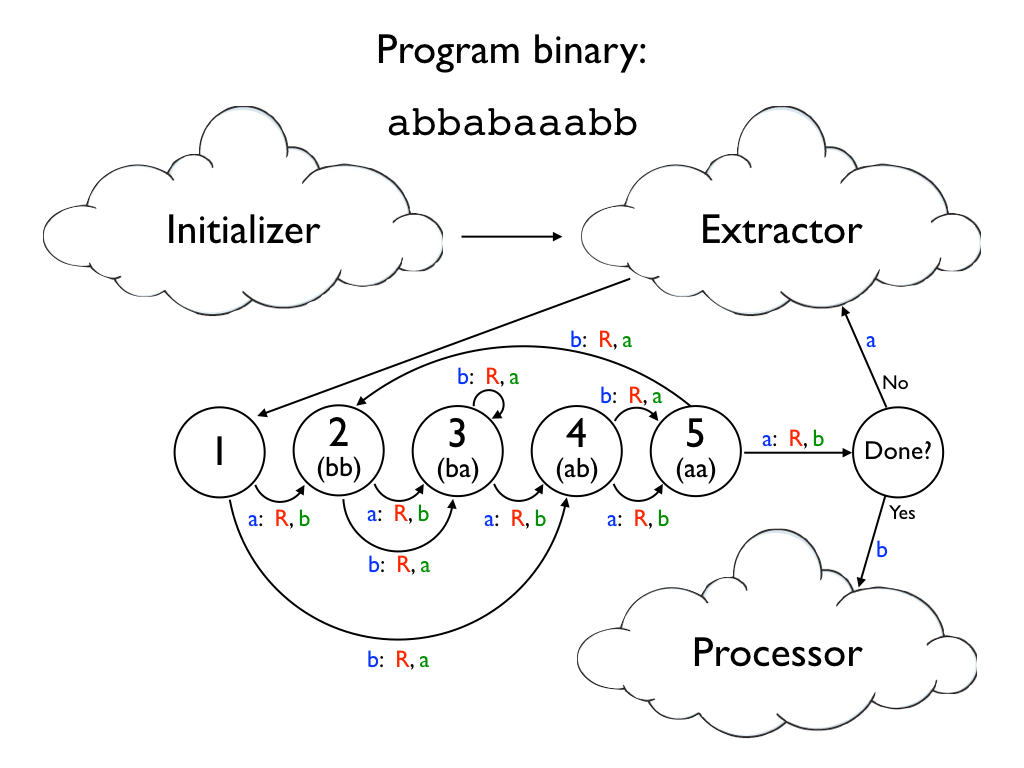
\includegraphics[scale=0.25]{figs/introspectprog.png}
\caption{An introspective implementation of the printer. \ In this example, the hypothetical program is $k=10$ bits long, and so the word size must be 2 (since $w=2$ is the largest $w$ such that $w2^w \le 10$). \ There are therefore $n_w = \left \lceil{\frac{k}{w}}\right \rceil = 5$ data states, each encoding two bits. \ The \texttt{b} transitions carry the information about the encoding; note that each one only points to one of the last four data states. \ The last four data states have in parentheses what word we mean to encode if we point to them. \label{fig:introspectprog}}
\end{center}
\end{figure}

On closer examination, however, this approach is quite wasteful for all but the smallest binary files. \ Every \texttt{a} transition points to the next state in the sequence, and none of the \texttt{b} transitions are used at all! \ Indeed, the only information-bearing part of the state is the single bit contained in the choice of which symbol to write. \ But in theory, far more information than that could be encoded in each state. \ In a machine with $n$ states, each state could contain $2(\log_2(n) + 1)$ bits of information, because each of its two transitions could point to any of the $n$ states, and write either an \texttt{a} or a \texttt{b} onto the tape. \ Of course, this is only in theory; in practice, to extract the information contained in therefore Turing machine's states and translate it into bits on the tape is nontrivial.

We will use a scheme originally conceived by Ben-Amram and Petersen and refined further and suggested to us by Luke Schaeffer. \ It does not achieve the optimal theoretical encoding described above, but is relatively simple to implement and understand, and is within a factor of $2$ of optimal for large binary strings. \ Schaeffer named Turing machines that use this idea \emph{introspective}.

Introspection works as follows. \ If the binary string contains $k$ bits, then let $w$ be the \emph{word size}. The word size $w$ takes the largest value it can such that $w2^w \le k$. \ We can split the binary string into $n_w = \left \lceil{\frac{k}{w}}\right \rceil$ \emph{words} of $w$ bits each (we can pad the last word with copies of the blank symbol). \ In our scheme, each word in the bit-string is represented by a \emph{data state}. \ Each data state points to the state representing the next word in the sequence for its \texttt{a} transition, but which state the \texttt{b} transition points to encodes the next word. \ Every \texttt{b} transition points to one of the last $2^w$ data states, thereby encoding $w$ bits of information.

Of course, the encoding is useless until we specify how to extract the encoded bit-string from the data states. \ The extraction scheme works as follows. \ To query the $i^\textrm{th}$ data state for the bits it encodes, we run the data states on the string $\texttt{a}^{i-1}\texttt{b}\texttt{a}^{\infty}$ (a string of $i-1$ \texttt{a}'s followed by a \texttt{b} in the $i^\textrm{th}$ position). \ After running the data states on that string, what remains on the tape is the string $\texttt{b}^{i-1}\texttt{a}\texttt{b}^r\texttt{a}^{\infty}$, assuming that the $i^\textrm{th}$ data state pointed to the $r^\textrm{th}$-to-last data state. \ Thus, what we're left with is essentially a unary encoding of the ``value'' of the word in binary. \ Thus, the job of the extractor is to set up a binary counter which removes one \texttt{b} at a time and increments the counter appropriately. \ Then, afterward, the extractor reverts the tape back to the form $\texttt{a}^i\texttt{b}\texttt{a}^{\infty}$, shifts all symbols on the tape over by $w$ bits, and repeats the process. \ Finally, when the state beyond the last data state sees a \texttt{b} on the tape, we know that the process has completed, and we can pass control to the processor. \ Figure~\ref{fig:introspectprog} shows the whole procedure.

How much have we gained by using introspection for encoding the program binary, instead of the na\"ive approach? \ It depends on how large the program binary is. \ Using introspection incurs an $O(\log k)$ \emph{additive} overhead, because we have to include the extractor in our machine. \ (Our implementation of the extractor takes $10w + 17$ states. It's possible to build a constant-size extractor, but it's not worth it for our value of $w$) \ In return, we save a \emph{multiplicative} factor of $w$ (which scales with $\log k$) on the number of data states needed.

This is plainly not worth it for the $10$-bit example binary shown in Figs.~\ref{fig:naiveprog} and~\ref{fig:introspectprog}. \ For that binary, we require $69$ additional states for the extractor in order to save $5$ data states. \ For real programs, however, it is worth it, as can be seen from the following table.

\begin{center}
    \begin{tabular}{||c c c c c c c||}
    \hline
    Program & Binary Size & $w$ & $n_w$ & Extractor Size & States (Na\"ive) & States (Introspective) \\ [0.5ex]
    \hline\hline
    Example TMD & 116 & 4 & 29 & 57 & 116 & 86 \\
    \hline
    Goldbach & 4,964 & 9 & 552 & 107 & 4,964 & 659 \\
    \hline
    Riemann & 9,532 & 10 & 1,024 & 117 & 9,532 & 1,141 \\
    \hline
    ZFC & 38,956 & 11 & 3,542 & 127 & 38,956 & 3,621 \\
    \hline
    \end{tabular}
\end{center}

One minor detail concerns the numbers presented for the Riemann program. \ Ordinarily, with a binary of size 9,532, we would opt to split the program into 1,060 words of 9 bits each plus a 107-state extractor, since 9 is the greatest $w$ such that $w2^w <$ 9,532. \ But because 9,532 is so close to the ``magic number'' 10,240, it's actually more parsimonious to pad the program with copies of the blank symbol until it's 10,240 bits long, and split it into 1,024 words of $10$ bits each plus a $117$-state extractor.


\section{The Processor}

The processor's job is to interpret the code written onto the tape and modify the variable registers and function stack accordingly. \ The processor does this by the following sequence of steps:  \\ \\
START:
\begin{enumerate}
\item Find the function call at the top of the stack. Mark the function $f$ in the code whose ID matches that of the top function call.
\item Read the current program counter. Mark the line of code $l$ in $f$ whose line number matches the program counter.
\item Read $l$. Depending on what type of command $l$ is, carry out one of the following three lists of tasks.
\end{enumerate}

\noindent IF $l$ IS AN EXPLICIT TAPE COMMAND:
\begin{enumerate}
\item Read the variable name off $l$. Index the variable name into the list of variables in the top function on the stack. This list of variables corresponds to the mapping between the function's local variables and the register names.
\item Match the indexed variable to its corresponding register $r$. Mark $r$. Read the symbol $s_r$ to the right of the head marker in that register.
\item Travel back to $l$, remembering the value of $s_r$ using states. Find and mark the reaction $x$ corresponding to the symbol. See what symbol $s_w$ should be written in response to reading $s_r$.
\item Travel back to $r$, remembering the value of $s_w$ using states. Replace $s_r$ with $s_w$.
\item Travel back to $x$. See which direction $d$ the head should move in response to reading $s_r$.
\item Travel back to $r$, remembering the value of $d$ using states. Move the head marker accordingly.
\item Travel back to $x$. See if a jump is specified. If a jump is specified, copy the jump address onto the program counter. Otherwise, increment the program counter by 1.
\item Go back to START.
\end{enumerate}

\noindent IF $l$ IS A FUNCTION CALL:
\begin{enumerate}
\item Write the function's name to the top of the stack.
\item For each variable in the function call, index the variable name into the list of variables in the top function on the stack. This list of variables corresponds to the mapping between the function's local variables and the register names. Push the corresponding register names in the order that they correspond to the variables in the function call.
\item Copy the current program counter to the return address of the newborn function call at the top of the stack.
\item Replace the current program counter with 0 (meaning ``read the first line of code'').
\item Go back to START.
\end{enumerate}

\noindent IF $l$ IS A RETURN STATEMENT:
\begin{enumerate}
\item Replace the current program counter with $f$'s return address.
\item Increment the program counter by 1.
\item Erase the call to $f$ from the top of the stack.
\item Check if the stack is now empty. If so, halt.
\item Go back to START.
\end{enumerate}


\end{document}